%Para este capítulo se usará la abreviatura "conex".
\chapter{Conexión}
\label{conex}
La noción de conexión es otra más de las nociones que ya conocíamos en $\R^n$ y espacios métricos en general y que pueden generalizarse a un espacio topológico arbitrario. En este capítulo formalizaremos la noción intuitiva de estar hecho ``de una sola pieza''. Asimismo también trabajaremos sobre el concepto de ``pieza indivisible'' de algo, o, dicho más finamente, ``componente conexa''. 
\section{Definición y propiedades}
Comencemos nuestra nueva andadura definiendo formalmente la idea de conexión y presentando algunos resultados bastante potentes.

\begin{defi}[Conexión]
	Un espacio topológico $(\X,\T)$ es \tbi[espacio!conexo|see{conexo}]{conexo} \indexg{conexo} si no lo podemos particionar con dos abiertos. Dicho de otra manera, un espacio es conexo si no unión de dos abiertos disjuntos no vacíos.
	
	Escrito de forma conjuntista, no existen $\U$ y $\V$ abiertos tales que $U\cap V=\emptyset$ y $\X=U\cup V$.
\end{defi}

\begin{obs}[Conexión en subespacios]
	De nuevo, como ocurría con la compacidad, la conexión en un subconjunto no necesita una definición alternativa. En efecto, dado un subespacio $\Y\subset\X$, diremos que $\Y$ es conexo si lo es entendido como un espacio topológico equipado con la topología relativa.
\end{obs}
La siguiente proposición bien podría ser una observación inmediata, no obstante es extremadamente útil y nos acerca a la idea que de vez en cuando hemos dejado caer acerca a la relación de los clopens con la conexión.
\begin{prop}[Definiciones equivalentes]
	Sea un espacio topológico $\X$. Las siguientes afirmaciones son equivalentes:
	\begin{enumerate}
		\item $\X$ no es conexo.
		\item $\X$ es unión de dos cerrados disjuntos no vacíos.
		\item $\X$ posee dos clopens no triviales.
	\end{enumerate}
\end{prop}
\begin{proof}
	Si $\X$ es disconexo es claro que podemos escribir $\X$ como unión disjunta de dos abiertos no triviales $\X=U\cup V$. Como $U$ es abierto, su complementario, $V$, será cerrado, luego $V$ será un clopen. Análogamente, como $V$ es abierto, su complementario, $U$, será cerrado, luego $U$ es también un clopen.
\end{proof}
Para ir calentando daremos una caracterización de los conexos de la recta real $\R$. La demostración de la siguiente proposición simplifica brutalmente a la que habitualmente se ve en la literatura y es debida a Diego Chicharro.
\begin{defi}[Intervalo]
	Un subconjunto no vacío $A\subset\R$ se dice \tbi{intervalo} si dados dos puntos $a,b\in A$ y un tercero $c\in\R$ que cumple que $a\leq c\leq b$, entonces $c\in A$. 
\end{defi}
\begin{prop}[Conexos de la recta]
	Un conjunto $A\subset \R$ es conexo si y solo si es un intervalo. 
\end{prop}
\begin{proof}
	Demostremos ambas implicaciones.
	\begin{enumerate}
		\item[\bra] Sea $A$ conexo de $\R$ que no sea un intervalo, entonces habrá dos puntos $a,b\in A$ para cuales podemos elegir un $c$ entre $a$ y $b$ tal que $c\not\in A$. Dicho esto, considerando los conjuntos $U:=(-\infty,c)\cap A$ y $V:=(c,\infty)\cap A$ es claro que son abiertos disjuntos de $A$ que cubren a $A$, luego $A$ no es conexo. 
		\item[\bla] Sea $A$ un intervalo. Si no fuera conexo, podría particionarlo en dos cerrados $F$ y $H$. Tomemos pues dos puntos, uno en cada abierto de la partición $a\in F$ y $b\in H$, supongamos sin pérdida de generalidad que $a<b$. Como $A$ es un intervalo, dados dos puntos de $A$, contiene a todos los que haya en medio, en particular $[a,b]\subset A$.
		
		Consideremos pues $H\cap[a,b]\not=\emptyset$, que, al ser intersección de cerrados es cerrado, y, por tanto, contiene a todos sus puntos de acumulación, en particular, al ser acotado contiene a su ínfimo, al que llamaremos $\eta$.
		
		Llegados a este punto, si $\eta=a$ entonces $a$ estará en los dos cerrados de la partición a la vez, lo cual es absurdo, precisamente por ser una partición. Esto obliga a que $\eta > a$, luego $[a,\eta)\cap H=\emptyset$ asique $[a,\eta)\subset F$. Al ser $F$ cerrado es claro que $[a,\eta]\subset F$. Pero esto es absurdo porque entonces $\eta$ estaría tanto en $F$ como $H$, que son conjuntos disjuntos.\qedhere
	\end{enumerate}
\end{proof}
Ahora, vamos a repasar brevemente las propiedades que ya conocíamos de conjuntos conexos en espacios métricos que siguen siendo válidas en estos mundos abstrusos.

\begin{prop}[Imagen continua]
	\label{conex_prop_im_continua}
	La imagen continua de un conexo es un conexo.
\end{prop}
\begin{proof}
	Sea $\X$ conexo y $f:\X\to f(\X)=:\Y$ continua. Veamos que $\Y$ es conexo. Razonemos pues por contradicción.
	
	Si $\Y$ no fuera conexo, tendría un clopen no trivial (ni el vacío ni el total), llamémoslo $A$. Entonces por ser $f$ continua, $f^{-1}(A)$ también es un clopen.
	
	Al ser $f$ sobreyectiva, $f(f^{-1}(A))=A\subsetneq f(\X)$, luego $f^{-1}(A)$ no puede ser ni el vacío ni el total, siendo así un clopen no trivial, entrando en contradicción con la conexión de $\X$.
\end{proof}

A continuación presentamos un teorema conocido en algunos lugares remotos como el teorema del pivote, aunque bien podría llamarse el teorema MacGyver.
\begin{theo}[Teorema de pivote]
	\label{conex_theo_pivote}
	Sea $\{A_i\}_{i\in I}$ una familia de conexos de $\X$ con intersección no vacía, es decir, hay un punto $a$ contenido en $\bigcap_{i\in I} A_i$.
	
	Entonces, la unión de la familia, $C:=\bigcup_{i\in I} A_i$ es conexo.
\end{theo}
\begin{proof}
	Veamos que $C$ no tiene clopens no triviales, para ello, supongamos que $S$ es un clopen de $C$. Al ser $S$ un clopen de $C$, por topología relativa, $S\cap A_i$ es un clopen de $A_i$. Ahora, como $A_i$ es conexo, $S\cap A_i$ tiene que ser necesariamente el vacío o el total, para cada $i\in I$.
	
	Si hubiera un $i_0\in I$ tal que $S\cap A_{i_0}=A_{i_0}$, como hay un $a$ en la intersección de la familia, $a\in A_{i_0}$, luego $a\in S$. Por tanto $S$ corta a todos los conjuntos de la familia, y, como dijimos antes, es un clopen en todos ellos, luego no queda más remedio que $S\cap A_i=A_i$ para todo $i\in I$. Siendo pues $S=C$.
	
	Por otra parte, si $S$ no corta a ninguno de los conjuntos de la familia es claro que es el vacío. 
\end{proof}

Este teorema es extremadamente útil para garantizar la conexión de un sinnúmero de conjuntos, y genera un gran abanico de corolarios y consecuencias (de ahí que le hayamos bautizado como el teorema MacGyver). Detallemos algunas variantes y consecuencias de este fantástico teorema.

\begin{cor}[Intersecciones dos a dos]
	\label{conex_cor_pivote_corte_comun}
	Sea $\{A_i\}_{i\in I}$ una familia de conexos que cumple que uno de ellos, digamos $A_{i_0}$, corta a todos los demás. Es decir, $A_{i_0}\cap A_i\not=\emptyset$ para todo $i\in I$.
	
	Entonces, la unión de la familia, $\bigcup_{i\in I} A_i$ es conexo.
\end{cor}
\begin{proof}
	Como $A_i\cap A_{i_0}\neq\emptyset$ por hipótesis, podemos aplicar el teorema del pivote a la familia $\{A_i,A_{i_0}\}$ para cada $i\in I$, y por tanto cada $A_{i_0}\cup A_i$ es conexo. Ahora, escribiendo
	\[\bigcup_{i\in I} A_i = \bigcup_{i\in I} (A_i\cup A_{i_0})\]
	tenemos que como la familia $\{A_i\cup A_{i_0}\midc i\in I\}$ tiene a $A_{i_0}$ por intersección, su unión (que coincide con la que queremos), por el teorema del pivote es conexa.
\end{proof}
\begin{obs}[Intersecciones dos a dos]
	En particular, la misma prueba del corolario \ref{conex_cor_pivote_corte_comun} tomando un $i_0\in I$ arbitrario sirve para una familia de conexos tal que su intersección dos a dos sea no vacía, es decir, $A_i\cap A_j\not=\emptyset$ para cualquier par de conjuntos de la familia.
\end{obs}
Como a veces la visión espacial brilla por su ausencia brindamos dos dibujos con ejemplos de familias de conexos que verifican las condiciones del corolario \ref{conex_cor_pivote_corte_comun}.
\begin{figure}[h!]
	\centering
	\subfigure[El corro de la patata]{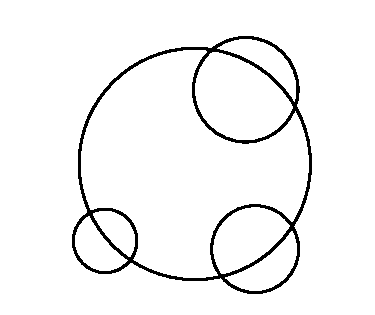
\includegraphics[scale = 0.4]{img/pivote_variante1}}
	\subfigure[El símbolo anarquista]{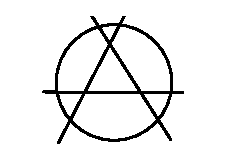
\includegraphics[scale = 0.8]{img/pivote_variante2}}
	\caption{Ilustración de conjuntos en las hipótesis de \ref{conex_cor_pivote_corte_comun}.}
\end{figure}

\begin{cor}[Cadenas]
	Sea una cadena finita $\{A_i\}_{i=1}^n$ de conexos, es decir, que verifica que $A_i\cap A_{i+1}\not=\emptyset$. Entonces $\bigcup_{i=1}^n A_i$ es conexo.
\end{cor}
\begin{proof}
	Por inducción, es claro que aplicando el teorema del pivote la cadena de dos eslabones $A_1\cup A_2$ es conexa, si suponemos que la cadena de $n$ eslabones es conexa, por el teorema del pivote, la de $n+1$ eslabones $A_{k+1}\cup\bigcup_{i=1}^k A_i$ lo será también.
\end{proof}
\begin{figure}[H]
	\centering
	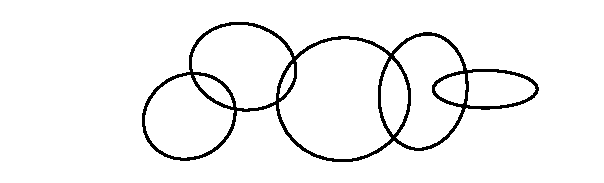
\includegraphics[scale = 0.5]{img/pivote_variante3}
	\caption{Ilustración de una cadena de conexos}
\end{figure}
\begin{obs}
	El corolario anterior también se verifica si la sucesión de conjuntos es numerable, pero no lo vamos a probar aquí.
	% AQUÍ VIENE PROBADO http://dbfin.com/topology/munkres/chapter-3/section-23-connected-spaces/problem-2-solution/
\end{obs}

El siguiente resultado, aunque también es consecuencia del teorema del pivote \ref{conex_theo_pivote}, es más que un mero corolario y merece la categoría de teorema por sí mismo.

\begin{theo}[Sandwich]\label{conex_teo_adherencia_conexa}
	Sea $A$ conexo y $B$ un conjunto emparedado entre $A$ y su adherencia, es decir, $A\subset B\subset\adher{A}$. Entonces $B$ es conexo. En particular, $\adher{A}$ es conexo.
\end{theo}
\begin{proof}
	Podemos poner nuestro conjunto $B$ de forma amigable para usar el teorema del pivote.
	\[B=\bigcup_{b\in B\setminus A} (A\cup\{b\}) \]
	como la intersección de la familia es no vacía, entonces basta probar que cada $A\cup\{b\}\subset\adher{A}$ es conexo, pues en ese caso el teorema del pivote \ref{conex_theo_pivote} nos garantiza la conexión de $B$.
	
	Si hubiera un clopen no trivial $C\subset A\cup\{b\}$, entonces, $C\cap A$ sería un clopen en $A$. Como $A$ es conexo, $C\cap A$ debe ser el vacío o el total.
	\begin{itemize}
		\item Si es el vacío, entonces $C=\{b\}$ y por tanto $\{b\}$ es abierto, luego, como el entorno $\{b\}$ de sí mismo no corta con $A$, $b\not\in\adher{A}$, lo cual es una contradicción.
		\item Si es el total, $C=A$ y por tanto $A$ es cerrado, pero $b\not\in A=\adher{A}$, que de nuevo es una contradicción. \qedhere
	\end{itemize}
\end{proof}

Recojamos los frutos de nuestra cosecha con un ejemplo, pero antes presentemos unas definiciones que harán más ágil nuestro discurrir.
\begin{defi}[Segmento]
	En $\R^n$ un segmento que une dos puntos $a$ y $b$ es el conjunto $\{ta+(1-t)b\midc t\in[0,1]\}$, que puede interpretarse como la imagen de la interpolación lineal entre $a$ y $b$, que definimos en la ecuación \eqref{interpolacion}.
\end{defi}
\begin{defi}[Convexo]
	En $\R^n$, se dice que un conjunto es \tbi{convexo} si para cada par de puntos $a,b\in E$, el segmento que los une también está en el conjunto.
\end{defi}
\begin{defi}[Estrellado]
	En $\R^n$ definimos conjunto \tbi{estrellado} como un conjunto en el que existe un punto tal que el segmento de él a cualquier otro está en el conjunto.
\end{defi}

\begin{exa}[Miscelánea] Veamos algunos ejemplos de conjuntos conexos:
	\begin{enumerate}
		\item Los segmentos son conexos por ser la imagén continua de $[0,1]$, que es conexo, por la interpolación lineal, que es continua.
		\item Si un conjunto es convexo entonces es estrellado, y si es estrellado entonces es conexo. Además, las implicaciones recíprocas no se verifican. En resumen
		\[\text{Convexo}\ra\text{Estrellado}\ra \text{Conexo}\]
		
		En efecto, si $A$ es convexo tomando cualquier punto como ``centro de la estrella'' se deduce que $A$ es estrellado.
		
		Asimismo, si $A$ es estrellado se puede escribir como
		\[A=\bigcup_{a\in A} [a_0, a]\]
		para cierto $a_0\in A$. Cada segmento $[a_0,a]$ es conexo, y, por tanto, por el teorema del pivote, como todos comparten el punto $a_0$, su unión es conexa.
		
		Nótese que ni la convexidad ni ser estrellado son propiedades topológicas; ambas son propiedades vectoriales: su definición solo tiene sentido en un espacio que, al menos, tenga estructura de espacio vectorial.
		
		\item Una circunferencia en $\R^2$ es conexa, pero no es estrellada. En efecto, es conexa por ser la imagen de $[0,2\pi]$ por la aplicación $t\mapsto (\cos t, \sen t)$.
		
		\item El grafo de la función $\sen\frac{1}{x}$ para $x>0$, que escribimos:
		\[C = \left\{\left(x,\sen\frac{1}{x}\right)\midc x>0\right\}\]
		es conexo por ser la imagen continua de $(0,\infty)$ por la aplicación:
		\[x\mapsto \left(x,\sen\frac{1}{x}\right)\]
		
		Lo que es más interesante, para cualquier $a\in [-1,1]$ se verifica que $\{(0,a)\}$ es adherente a $C$ (es relativamente fácil de comprobar) y por tanto que $C\cup\{(0,a)\}$ es conexo.
		\begin{figure}[H]
			\centering
			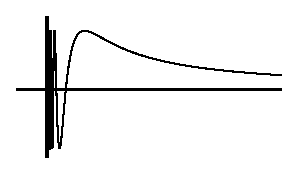
\includegraphics[scale = 0.8]{img/funcionsen1x}
			\caption{Ilustración de la gráfica de $\sen(1/x)$}
		\end{figure}
		
		\item Consideramos el conjunto:
		\begin{equation}\label{lineas}C = \big(\{0\}\times (0,1]\big) \cup \left(\bigcup_{n\in\N} [0,1]\times\left\{\frac{1}{n}\right\}\right) \end{equation}
		\begin{figure}[H]
			\centering
			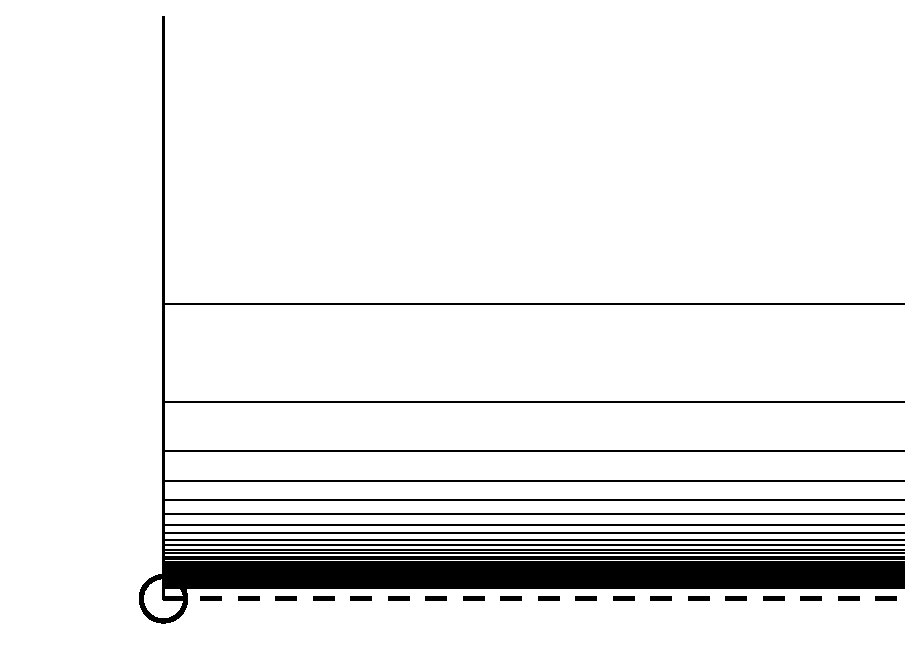
\includegraphics[scale = 0.2]{img/lineas}
			\caption{Ilustración del conjunto de la ecuación \eqref{lineas}}
		\end{figure}
		que es unión de segmentos horizontales cada vez más juntos y de un segmento vertical. Este es trivialmente conexo por el corolario \ref{conex_cor_pivote_corte_comun}. Lo particular es que si unimos a $C$ el segmento horizontal:
		\[(0,1)\times\{0\}\]
		sigue siendo conexo por ser adherencia de $C$ (¡compruébese!). 
\qedhere
	\end{enumerate}
\end{exa}

Completamos esta sección con una propiedad interesante garantizada por la conexión.

\begin{lem}[Cadena]
	Sea $\X$ conexo y $\{U_i\}_{i\in I}$ un recubrimiento por abiertos de $\X$. Dos puntos cualesquiera $x,y\in\X$ se pueden conectar mediante una cadena finita de abiertos del recubrimiento.
\end{lem}

\begin{proof}
	Sea $A=\{z\in\X \midc \text{existe una cadena de } x \text{ a } z \}$. $A$ es claramente no vacío, puesto que $x\in A$. Por ende, nuestro objetivo será ver que $\X=A$. Una forma de hacerlo será ver que $A$ es un clopen, ya que si lo fuera, por conexión de $\X$ y por ser $A$ no vacío $A$ tendría que ser el total.
	\begin{itemize}
		\item Veamos que $A$ es abierto. En efecto, dado $z\in A$, queremos ver que existe un abierto $U$ tal que $z\in U\subset A$. Si tomamos el último abierto $U$ de la cadena que une $x$ y $z$ hemos ganado, ya que $U\subset A$, ya que todo punto de $U$ queda unido con $x$ con la misma cadena que $z$.
		
		\item Ahora la clausura. En efecto, si $z\in\adher{A}$, entonces habrá un abierto $U_{i_0}$ tal que $U_{i_0}\cap A\not=\emptyset$. Considerando un punto $y$ de la intersección, como $y$ está en $A$, hay una cadena de $x$ a $y$. Uniendo $U_{i_0}$ a la cadena obtenemos una cadena de $x$ a $z$, y por tanto $z\in A$, luego $A=\adher{A}$. \qedhere
	\end{itemize}
\end{proof}
Este último resultado tiene una aplicación muy importante en los espacios euclídeos usuales.
\begin{defi}[Poligonal]
	Una \tbi{poligonal} en $\R^n$ es un conjunto $\Gamma$ de la forma\begin{equation*}
		\Gamma=[x_0,x_1]\cup[x_1,x_2]\cup\dots\cup[x_{n-2},x_{n-1}]\cup[x_{n-1},x_n]
	\end{equation*}
	Donde $[x_i,x_j]$ representa el segmento que une a los puntos $x_i$ y $x_j$. Nótese que por la variante de las cadenas del teorema del pivote una poligonal es conexa.
\end{defi}
\begin{defi}[Conexión por poligonales]
	Un conjunto $A\subset\R^n$ se dice \tbi[conexo!por poligonales]{conexo por poligonales} si dados dos puntos cualesquiera $x,y\in A$, hay una poligonal $\Gamma$ contenida en $A$ que une a $x$ y a $y$.
\end{defi}
\begin{obs}[Conexión y conexión por poligonales]
	Todo conjunto conexo por poligonales es conexo. En efecto, si tomamos un punto $a$ de $A$ y consideramos la familia de poligonales (conexos) que conectan a $a$ con el resto de puntos de $A$, tenemos que dicha familia tiene a $\{a\}$ por intersección, luego podemos aplicar el teorema del pivote, obteniendo que la unión de la familia, que es $A$, es conexa.
\end{obs}
\begin{obs}[Abiertos y conexión por poligonales]
	Podemos recubrir cualquier abierto conexo de $\R^n$ con bolas (véase el lema \ref{etop_lem_otrasProp}), y, por tanto existe una cadena de bolas que une cualquier par de puntos.
	
	Si tomamos un punto en cada intersección entre bolas consecutivas de la cadena y consideramos los segmentos que los unen, tengo una poligonal que conecta los dos puntos.
	
	De esta forma, para abiertos de $\R^n$ la conexión y la conexión por poligonales son nociones equivalentes.
\end{obs}

\section{Componentes conexas}

Al igual que ocurría con la compacidad, sería deseable que todos los espacios fuesen conexos. Dado que esto no se da, nos conformaremos con quedarnos con los subconjuntos conexos del espacio. Surge así la idea de componente conexa que definimos a continuación. Aunque parezca que esto no es una ventaja, es tremendamente útil a la hora de estudiar, por ejemplo, si dos espacios son homeomorfos.

\begin{defi}
	Un subconjunto $\Co\subset\X$ es una \tbi{componente conexa} si es un conjunto conexo maximal.
\end{defi}

Una consecuencia inmediata de la definición es que, dado $x\in\X$,
\begin{equation}
	\Co(x)=\bigcup_{x\in A \text{ conexo}} A
\end{equation}
es una componente conexa, que denominaremos componente conexa de $x$.

En efecto, la unión no es vacía, pues el punto en sí es conexo. Además $x$ pertenece a la intersección de todos ellos. Como cada $A$ es conexo, basta aplicar el teorema del pivote para deducir que $\Co(x)$ es conexo. Por construcción es, además, maximal, ya que cualquier conexo que lo contenga, contiene a $x$ y, por tanto, está en la unión.

Cabe destacar que $\Co(x)$ es más que maximal, ya que cumple lo siguiente. Sea $E\subset\X$ conexo tal que $E\cap \Co(x)\not=\emptyset$. Entonces $E\cup \Co(x)$ es conexo y además $x\in E\cup \Co(x)$, por lo que $E\cup \Co(x)\subset \Co(x)$, es decir, $E\subset \Co(x)$.

Esto será muy utilizado de aquí en adelante, cualquier conexo que interseque con una componente conexa está contenido en ella.

\begin{obs}
	Nótese que hay varios punto con la misma componente conexa y que si el espacio es conexo, entonces es la componente conexa de todos los puntos.
\end{obs}

A continuación enunciamos y demostramos algunas propiedades de las componentes conexas.

\begin{lem}
	Sea $\X$ un espacio topológico, entonces:
	\begin{enumerate}
		\item Las componentes conexas son cerradas.
		
		\item Las componentes conexas son una partición del espacio.
		
		\item Si $\X$ es la unión disjunta de las componentes conexas, siendo estas finitas, entonces las componentes conexas son abiertas.
		
		\item Si en $\X$ todo punto tiene un entorno conexo, entonces las componentes conexas de $\X$ son abiertas.
	\end{enumerate}
\end{lem}
\begin{proof}
	Vayamos con la demostración:
	\begin{enumerate}
		\item Sea $\Co(x)$ componente conexa. Como es conexo, por el teorema~\ref{T7:teo_adherencia_conexa} su adherencia es conexa, y por ser maximal $\Co(x)=\adher{\Co(x)}$.
		
		\item Es claro que
		\[\X=\bigcup_{x\in\X} \Co(x)\]
		Además, dadas dos componentes conexas, $\Co_1$ y $\Co_2$, si $\Co_1\cap\Co_2\not=\emptyset$ entonces $\Co_1\subseteq\Co_2$ y por ser maximales se da la igualdad.
		
		\item Por hipótesis $\X=\Co_1\cup\cdots\cup\Co_r$ siendo la unión disjunta. Entonces, para cada $i\in\{1,\cdots r\}$ se tiene que 
		\[\Co_i=\X\backslash (\Co_1\cup\cdots\cup\Co_{i-1}\cup\Co_{i+1}\cup\cdots\cup\Co_r)=\X\backslash \Co\]
		Como cada componente conexa es cerrada por 1, la unión finita es cerrada $\Co$, luego $C_i=\X\backslash \Co$ es abierto para todo $i$.
		
		\item Sea $\Co$ componente conexa de $\X$ y veamos que es entorno de todos sus puntos. Sea $x\in\Co$. Por hipótesis existe $\V$ entorno conexo de $x$, con lo cual $\V\cap\Co\not=\emptyset$. Esto implica que $x\in\V\subset\Co$, con lo que $\Co$ es entorno de $x$.
	\end{enumerate}
\end{proof}

%Tablas comportamiento topológico. Añado aquí también las de conexión por caminos, dado que no está aun el tema.

\section{Comportamiento de la conexión}
\section{Comportamiento de la local--conexión}

\begin{table}[h]
	\centering
	\begin{tabular}{l|l|l|l|l|}
		\cline{2-5}
		& \textbf{Subespacios}    & \textbf{Cociente}       & \textbf{Producto}       & \textbf{Suma}           \\ \hline
		\multicolumn{1}{|c|}{\textbf{Conexión}} & \multicolumn{1}{c|}{No} & \multicolumn{1}{c|}{Sí*} & \multicolumn{1}{c|}{Sí} & \multicolumn{1}{c|}{No} \\ \hline
	\end{tabular}
	\caption{Tabla resumen de conexión.}
	\label{Tabla_conexion}
\end{table}

\begin{table}[h]
	\centering
	\begin{tabular}{l|l|l|l|l|}
		\cline{2-5}
		& \textbf{Subespacios}                                                                      & \textbf{Cociente}       & \textbf{Producto}       & \textbf{Suma}           \\ \hline
		\multicolumn{1}{|c|}{\textbf{\begin{tabular}[c]{@{}c@{}}Local\\ conexión\end{tabular}}} & \multicolumn{1}{c|}{\begin{tabular}[c]{@{}c@{}}Sí, en el caso\\ de abiertos\end{tabular}} & \multicolumn{1}{c|}{Sí} & \multicolumn{1}{c|}{Sí} & \multicolumn{1}{c|}{Sí} \\ \hline
	\end{tabular}
	\caption{Tabla resumen de local conexión}
	\label{Tabla_localconexion}
\end{table}

\begin{table}[h]
	\centering
	\begin{tabular}{c|c|c|c|c|}
		\cline{2-5}
		\multicolumn{1}{l|}{}                                                                                  & \multicolumn{1}{l|}{\textbf{Subespacios}}                             & \multicolumn{1}{l|}{\textbf{Cociente}} & \multicolumn{1}{l|}{\textbf{Producto}} & \multicolumn{1}{l|}{\textbf{Suma}} \\ \hline
		\multicolumn{1}{|c|}{\textbf{\begin{tabular}[c]{@{}c@{}}Conexo por\\ caminos\end{tabular}}}            & No                                                                    & Sí                                     & Sí                                     & No                                 \\ \hline
		\multicolumn{1}{|c|}{\textbf{\begin{tabular}[c]{@{}c@{}}Localmente conexo\\ por caminos\end{tabular}}} & \begin{tabular}[c]{@{}c@{}}Sí, en el caso \\ de abiertos\end{tabular} & Sí                                     & Sí                                     & Sí                                 \\ \hline
	\end{tabular}
	\caption{Tabla resumen de conexión por caminos}
	\label{Tabla_conexion_caminos}
\end{table}

\begin{figure}[h!]
	\centering
	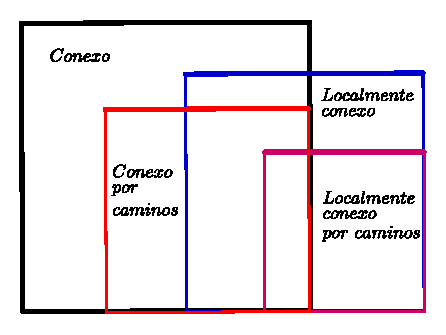
\includegraphics[scale = 1]{img/Comparacion_conexion}
\end{figure}
